\subsection{Упражнение 1}

Оценка вокального чирпа для нескольких времён начала сегмента. Возьмем пение птицы

\begin{lstlisting}[language=Python]
if not os.path.exists('456440__inspectorj__bird-whistling-robin-single-13.wav'):
    !wget https://github.com/hotnotHD/Telecom/raw/main/456440__inspectorj__bird-whistling-robin-single-13.wav

wave = read_wave('456440__inspectorj__bird-whistling-robin-single-13.wav')

wave.normalize()
wave.make_audio()

duration = 0.01
segment1 = wave.segment(start=0.24, duration=duration)
segment1.plot()
segment2 = wave.segment(start=0.26, duration=duration)
segment2.plot()
segment3 = wave.segment(start=0.28, duration=duration)
segment3.plot()
\end{lstlisting}

\begin{figure}[H]
	\begin{center}
		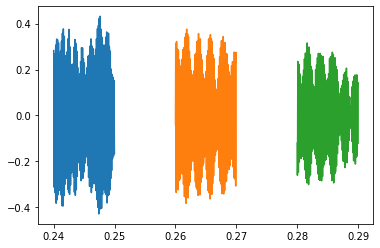
\includegraphics[scale=1]{fig/lab05/lab05_01.png}
		\caption{График выбранных сегментов}
	\end{center}
\end{figure}

Используем автокорреляцию для поиска высоты тона

\begin{lstlisting}[language=Python]
lags1, corrs1 = autocorr(segment1)
plt.plot(lags1, corrs1, color='green')
decorate(xlabel='Lag (index)', ylabel='Correlation', ylim=[-1, 1])

lags2, corrs2 = autocorr(segment2)
plt.plot(lags2, corrs2)
decorate(xlabel='Lag (index)', ylabel='Correlation', ylim=[-1, 1])

lags3, corrs3 = autocorr(segment3)
plt.plot(lags3, corrs3, color='red')
decorate(xlabel='Lag (index)', ylabel='Correlation', ylim=[-1, 1])
\end{lstlisting}

\begin{figure}[H]
	\begin{center}
		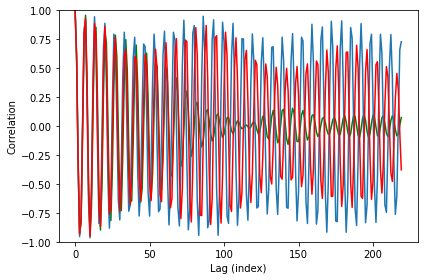
\includegraphics[scale=1]{fig/lab05/lab05_02.png}
		\caption{Автокорреляция сигналов}
	\end{center}
\end{figure}

Вычислим значения Lags, периоды и Fmax

\begin{lstlisting}[language=Python]
low, high = 50, 200
lag1 = np.array(corrs1[low:high]).argmax() + low

low, high = 50, 200
lag2 = np.array(corrs2[low:high]).argmax() + low

low, high = 50, 200
lag3 = np.array(corrs3[low:high]).argmax() + low

lag1, lag2, lag3

(54, 86, 88)

period1 = lag1 / segment1.framerate
period2 = lag2 / segment2.framerate
period3 = lag3 / segment3.framerate
period1, period2, period3

(0.0012244897959183673, 0.0019501133786848073, 0.00199546485260771)

frequency1 = 1 / period1
frequency2 = 1 / period2
frequency3 = 1 / period3
frequency1, frequency2, frequency3

(816.6666666666667, 512.7906976744185, 501.1363636363636)
\end{lstlisting}


\subsection{Упражнение 2}
Пример кода в chap05.ipynb показывает, как использовать автокорреляцию для оценки основной частоты периодического сигнала. Инкапсулируйте этот код в функцию estimate_dundamental, и используйте ее для отслеживания высоты тона записанного звука. Для тестирования возьмем тот же звук сирены

Инкапсулируем код для оценки основной частоты периодического сигнала из chap05.ipynb в функцию estimate_dundamental

\begin{lstlisting}[language=Python]
wave.make_audio()
\end{lstlisting}

Построим спектограмму

\begin{lstlisting}[language=Python]
wave.make_spectrogram(2048).plot(high = 4200)
\end{lstlisting}

\begin{figure}[H]
	\begin{center}
		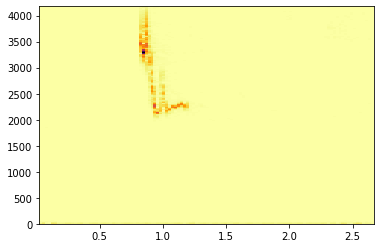
\includegraphics[scale=1]{fig/lab05/lab05_03.png}
		\caption{Спектрограмма записи}
	\end{center}
\end{figure}

Используем функцию estimate_fundamental из главы 5. Самый высокий пик в функции автокорреляции был отслежен с помощью выставления диапазона дагов для поиска от 70 до 200

\begin{lstlisting}[language=Python]
def estimate_fundamental(segment, low=70, high=200):
    lags, corrs = autocorr(segment)
    lag = np.array(corrs[low:high]).argmax() + low
    period = lag / segment.framerate
    frequency = 1 / period
    return frequency
    
duration = 0.01
segment = wave.segment(start=0.1, duration=duration)
freq = estimate_fundamental(segment)
freq

383.4782608695652
\end{lstlisting}

В цикле отследим пик по всему звуку. ts - это середина каждого сегмента

\begin{lstlisting}[language=Python]
step = 0.05
starts = np.arange(0.0, 1.4, step)

ts = []
freqs = []

for start in starts:
    ts.append(start + step/2)
    segment = wave.segment(start=start, duration=duration)
    freq = estimate_fundamental(segment)
    freqs.append(freq)
\end{lstlisting}

Синяя линия на графике наложена на спектограмму и показывает отслеживание высоты тона

\begin{lstlisting}[language=Python]
wave.make_spectrogram(2048).plot(high = 900)
plt.plot(ts, freqs, color='blue')
decorate(xlabel='Time (s)', ylabel='Frequency (Hz)')
\end{lstlisting}

\begin{figure}[H]
	\begin{center}
		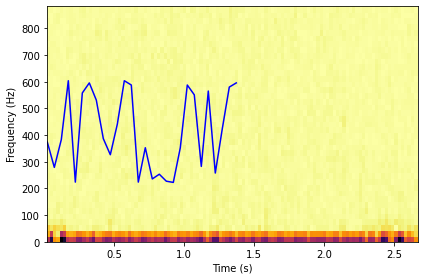
\includegraphics[scale=1]{fig/lab05/lab05_04.png}
		\caption{Результат}
	\end{center}
\end{figure}


\subsection{Упражнение 3}

Возьмем данные о BitCoin из прошлой лабораторной работы и вычислим для этих данных автокорреляцию цен

\begin{lstlisting}[language=Python]
if not os.path.exists('BTC_USD_2013-10-01_2020-03-26-CoinDesk.csv'):
    !wget https://github.com/AllenDowney/ThinkDSP/raw/master/code/BTC_USD_2013-10-01_2020-03-26-CoinDesk.csv
    
import pandas as pd

df = pd.read_csv('BTC_USD_2013-10-01_2020-03-26-CoinDesk.csv', parse_dates=[0])
df

\end{lstlisting}

\begin{figure}[H]
	\begin{center}
		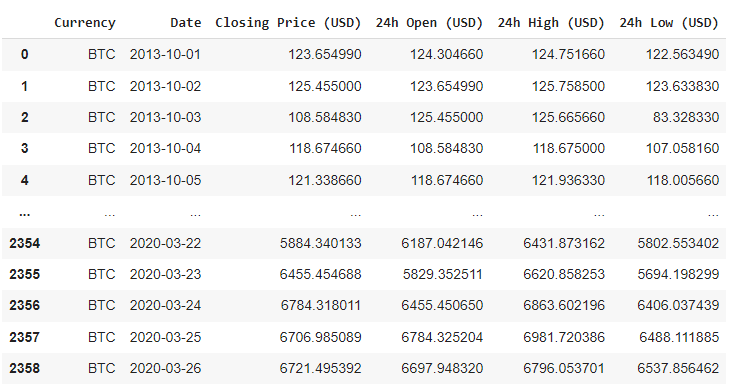
\includegraphics[scale=1]{fig/lab05/lab05_05.png}
		\caption{Таблица цены на BitCoin}
	\end{center}
\end{figure}

Вычислим автокорреляцию:

\begin{lstlisting}[language=Python]
ys = df['Closing Price (USD)']
ts = df.index

wave = Wave(ys, ts, framerate = 1)
wave.plot()
decorate(xlabel='Дни')
\end{lstlisting}

\begin{figure}[H]
	\begin{center}
		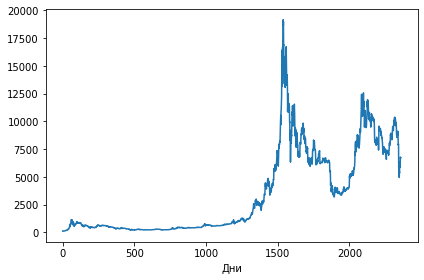
\includegraphics[scale=1]{fig/lab05/lab05_06.png}
		\caption{График цен на BitCoin}
	\end{center}
\end{figure}

\begin{lstlisting}[language=Python]
lags, corrs = autocorr(wave)
plt.plot(lags, corrs)
\end{lstlisting}

\begin{figure}[H]
	\begin{center}
		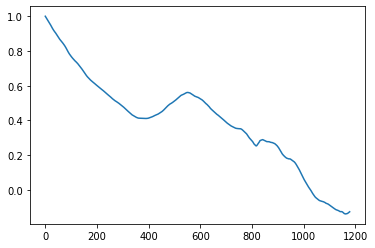
\includegraphics[scale=1]{fig/lab05/lab05_07.png}
		\caption{Автокорреляция функции цены на BitCoin}
	\end{center}
\end{figure}

Исходя из графика видно, что он постепенно снижается и похож на розовый шум. Также присутствует умеренная корреляция на 550 дне и 820. Теперь вычислим корреляцию на основе функции np.correlate, она не смещает и нормализует волну.

\begin{lstlisting}[language=Python]
corrs2 = np.correlate(wave.ys, wave.ys, mode = 'same')
lags = np.arange(-len(wave) // 2, len(wave) // 2)
plt.plot(lags, corrs2)
\end{lstlisting}

\begin{figure}[H]
	\begin{center}
		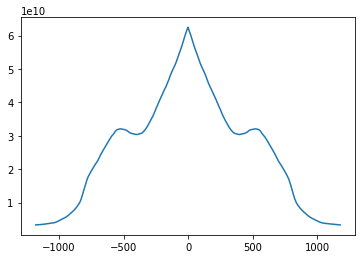
\includegraphics[scale=1]{fig/lab05/lab05_08.png}
		\caption{Автокорреляция функции цены на BitCoin при помощи np.correlate}
	\end{center}
\end{figure}

Вторая часть результатов (правая) соответствует положительными интервалам lags

\begin{lstlisting}[language=Python]
N = len(corrs2)
half = corrs[N//4:]
plt.plot(half)
\end{lstlisting}

\begin{figure}[H]
	\begin{center}
		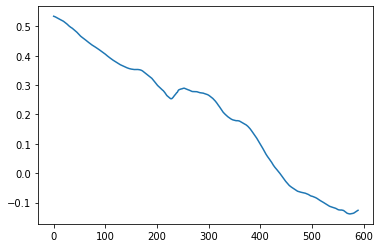
\includegraphics[scale=1]{fig/lab05/lab05_09.png}
		\caption{Правая часть результатов}
	\end{center}
\end{figure}


\subsection{Упражнение 4}

В репозитории Jupyter есть блокнот saxophone.inypb, в котором исследуется автокорреляция, восприятие высоты тона и явление, называемое подавленная основная. Прочтите этот блокнто и "погоняйте" примеры. Выберите другой сегмент записи и вновь поработайте с примерами

\begin{lstlisting}[language=Python]
if not os.path.exists('100475__iluppai__saxophone-weep.wav'):
    !wget https://github.com/AllenDowney/ThinkDSP/raw/master/code/100475__iluppai__saxophone-weep.wav
    
wave = read_wave('100475__iluppai__saxophone-weep.wav')
wave.normalize()
wave.make_audio()
\end{lstlisting}

Построим спектограмму

\begin{lstlisting}[language=Python]
wave.make_spectrogram(1024).plot(high = 3000)
decorate(xlabel='Time (s)', ylabel='Frequency (Hz)')
\end{lstlisting}

\begin{figure}[H]
	\begin{center}
		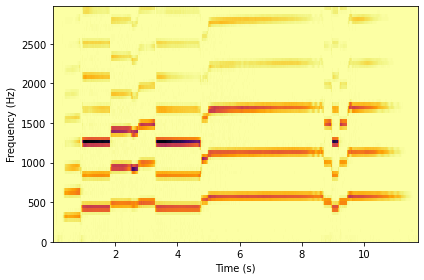
\includegraphics[scale=1]{fig/lab05/lab05_10.png}
		\caption{Спектрограмма звука}
	\end{center}
\end{figure}

На графике видна гармоническая структура во времени

Теперь возьмем некоторый сегмент и "прогоним" его через функции из блокнота

\begin{lstlisting}[language=Python]
segment = wave.segment(start=1, duration=0.2)
segment.make_audio()

spectrum = segment.make_spectrum()
spectrum.plot(high=4000)
decorate(xlabel='Frequency (Hz)', ylabel='Amplitude')
\end{lstlisting}

\begin{figure}[H]
	\begin{center}
		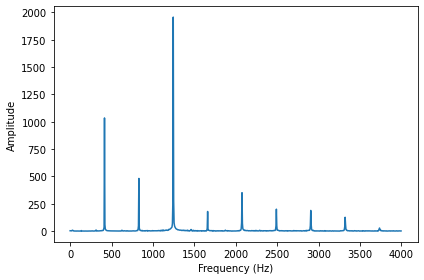
\includegraphics[scale=1]{fig/lab05/lab05_11.png}
		\caption{Спектр звука}
	\end{center}
\end{figure}

Данный спектр похож на спектр квадратного сигнала. Пики находятся на 1245, 415 и 830 Гц

\begin{lstlisting}[language=Python]
spectrum.peaks()[:10]

[(1956.703292712428, 1245.0),
 (1034.570299739157, 415.0),
 (481.52480153206335, 830.0),
 (351.0776583833776, 2075.0),
 (275.4196733573752, 1250.0),
 (264.72288947314, 1240.0),
 (200.51232139688983, 2490.0),
 (188.9737445345148, 2905.0),
 (179.39558697128783, 1660.0),
 (126.34825373317715, 3320.0)]
\end{lstlisting}

Теперь сравним наш сигнал с треугольным, у которого такая же низкая частота пика

\begin{lstlisting}[language=Python]
from thinkdsp import TriangleSignal

TriangleSignal(freq=415).make_wave(duration=0.2).make_audio()
\end{lstlisting}

Воспользуемся автокорреляцией для понимания основной частоты

\begin{lstlisting}[language=Python]
def autocorr2(segment):
    corrs = np.correlate(segment.ys, segment.ys, mode='same')
    N = len(corrs)
    lengths = range(N, N//2, -1)

    half = corrs[N//2:].copy()
    half /= lengths
    half /= half[0]
    return half
    
corrs = autocorr2(segment)
plt.plot(corrs[:500])
\end{lstlisting}

\begin{figure}[H]
	\begin{center}
		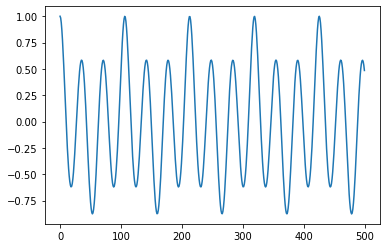
\includegraphics[scale=1]{fig/lab05/lab05_12.png}
		\caption{Автокорреляция}
	\end{center}
\end{figure}

Исходя из графика видны пики рядом c lag 100

Теперь найдем основную частоту

\begin{lstlisting}[language=Python]
estimate_fundamental(segment)

416.0377358490566
\end{lstlisting}

Попробуем убрать основной тон, что лучше воспринимать звук

\begin{lstlisting}[language=Python]
spec2 = segment.make_spectrum()
spec2.high_pass(600)
spec2.plot(high=5000)
decorate(xlabel='Frequency (Hz)', ylabel='Amplitude')
\end{lstlisting}

\begin{figure}[H]
	\begin{center}
		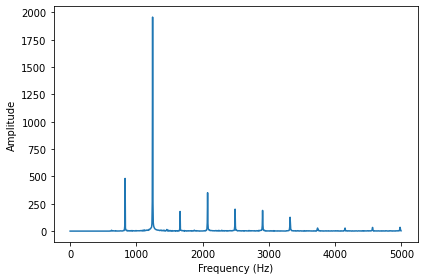
\includegraphics[scale=1]{fig/lab05/lab05_13.png}
		\caption{Спектр сигнала}
	\end{center}
\end{figure}

\begin{lstlisting}[language=Python]
segment2 = spec2.make_wave()
segment2.make_audio()
\end{lstlisting}

Звук воспринимается также

Это явление называется missing fundamental. Чтобы понять то, что мы слышим частоту, которой нет, можно снова использовать автокорреляцию.

\begin{lstlisting}[language=Python]
corrs = autocorr2(segment2)
plt.plot(corrs[:500])
\end{lstlisting}

\begin{figure}[H]
	\begin{center}
		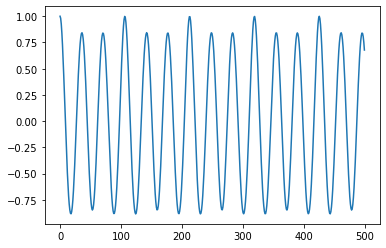
\includegraphics[scale=1]{fig/lab05/lab05_14.png}
		\caption{Автокорреляция}
	\end{center}
\end{figure}

\begin{lstlisting}[language=Python]
estimate_fundamental(segment2)

416.0377358490566
\end{lstlisting}

Получились одинаковые значения, так как более высокие компоненты сигнала являются гармониками 416Гц

Исходя из проведенных опытов можно сделать вывод, что восприятие выосты тона основано не только на спектральном анализе, но и на вычислении АКФ.


\subsection{Вывод}

В данной главе была изучена корреляция и её роль в сигналах. Также на пратике был обработан сигнал с "missing fundamental". Когда мы убирали основной тон, всё равно звук звучал также.